
\chapter{Observable to Study the Underlying Event}
\label{chap:ObservabletoStudytheUnderlyingEvent}

The UE are all the processes not associated with the primary hard scatter in an hadron-hadron collision.
\\
All the process described in the previous section: ISR and FSR, MPI, and BBR and their interactions with color exchanges among them, contribute to the Underlying Event (UE) in the proton-proton collision.
\\
The most of the observables to study the UE are sensible only to the sum of these contributions and not to the single ones so a good description of all this process and their interplay is really important.
\\
In this chapter these observables are introduced and 
described with more details.

\section{Minimum Bias Measurements and Underlying Event topology}

A Minimum Bias (MB) measurement is a collection of inelastic events with a loose event selection. The events are collected requiring the minimal interaction with the detector (the smallest possible bias). The most of the interaction in MB observation are soft, $p_T\lesssim2\ \mathrm{GeV}$. The study of the UE require at least one hard scattering ($p_T\gtrsim2\ \mathrm{GeV}$) presence, in fact the UE is given by the underlying activity to an hard scatter.
\\
To study the UE the topological structure of an hadron-hadron collision is used. The analysis is performed on an event-by-event basis. In the analysis the direction of the leading object is used to define regions in the $\eta-\phi$ space. Where $\eta$ is the pseudorapidity defined as $\eta=-\log{\tan\left(\frac{\theta}{2}\right)}$, while $\phi$ is the azimuthal angle in the $x-y$ plane. 
The last one is defined from the direction of the leading object as $\Delta\phi=\phi-\phi_{\text{leading}}$ .
%
\begin{figure}[!ht]
	\centering
	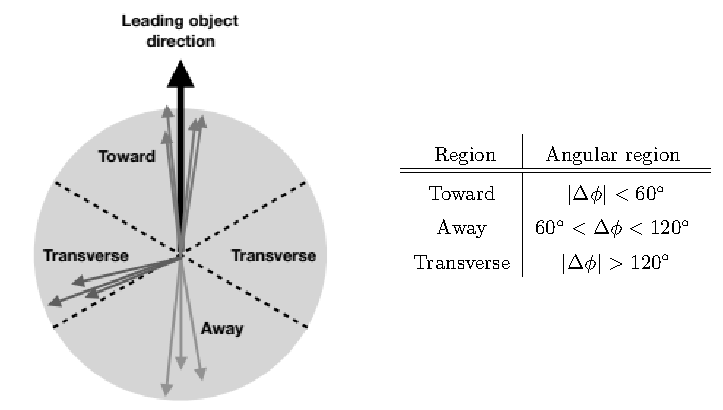
\includegraphics[width=0.8\textwidth]{{img/Regions.pdf}}
	\caption{This figure shows the four regions for the description of the UE on a event-by-event analysis. the angular values are shown in the table. The regions are defined starting from the leading object direction. The toward and away regions contain most of the contribution from the hard scattering (e.g. in a $t\overline{t}$ production event the two quark $t$ are located in these regions); while, the transverse region are the ones in between the twp other regions, these are the most important for the study of the UE.}
	\label{fig:Regions}
\end{figure}
%
\\
The regions classification is shown in \figRef{fig:Regions}, we have:
\begin{itemize}
	\item \textbf{Toward region}: the region that contains the leading object, this region contains the most of the particle produced by the hard interaction.
	\item \textbf{Away region}: this region contains the objects that recoil against the leading object, also this region contains mostly the particles produced by the hard interaction.
	\item \textbf{Transverse regions}: the two transverse regions are the most sensitive to UE.
\end{itemize}
The transverse regions are also separated in:
\begin{itemize}
	\item[--] \textbf{TransMAX}: This is the transverse region that contains the \textit{maximum} number of charged particles, or scalar $p_T$ sum of charged particles. This regions includes both MPI and hard-process contamination.
	\item[--] \textbf{TransMIN}: is the transverse region that contains the \textit{minimum} number of charged particles, or scalar-$p_T$ sum of charged particles. This region is the most  sensitive to MPI effects.
\end{itemize}

The leading object definition depend on the type of event under observation. 
The charged-particle with largest $p_T$ \cite{CMS-PAS-FSQ-15-007}, the dilepton system in Drell-Yan observation \cite{CMS:2012oqb, CMS:2017ngy} or $t\overline{t}$ events \cite{CMS:2018mdd} can all be used as leading object in the analyses for the UE event.
\\
So we are interest in studying the transMAX and transMIN region in particular the observable sensitive to UE in these regions are: the charged-particle density and the charged-particle scalar-$p_T$ sum density in the $\eta-\phi$ space

In an hadron-hadron collision with two jets productions it is observed that also the transverse regions activity increase with energy, as shown in \figRef{fig:UEpredictions_in_regions.png}, where the different color lines refer to different scales for the collision. Is observed that the away region ($60\leq |\Delta\phi|\leq 120$) at increasing energy for the collision become broader this is related to the increasing quantity of FSR.
\\
This increment in the transverse regions activity cannot be explained only by the increase of the FSR. To explain this rise one need to attribute activity in the transverse regions to MPI, extra scattering increasing with energy is related to the partons inside the hadrons that become denser packed when probed at higher energies. 

\begin{figure}[!ht]
	\centering
	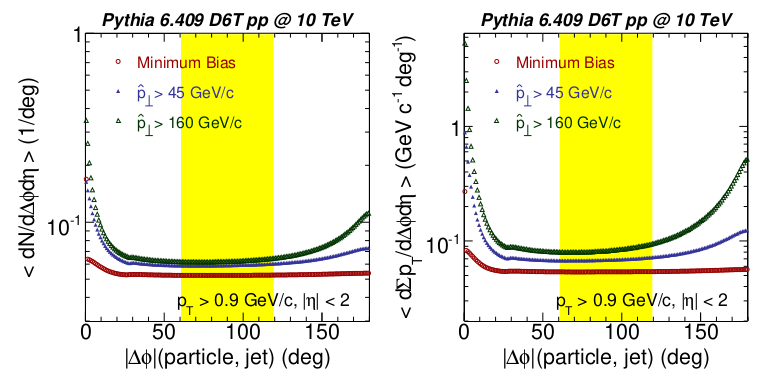
\includegraphics[width=0.8\textwidth]{{img/UEpredictions_in_regions.png}}
	\caption{A comparison between three different scales for the interaction. The multiplicity of charged particles (left) and the scalar-$p_T$ sum of charged particles (right) are simulated. The activity in the transverse regions increase due two effects: the FSR this is related to the broadening of the away region so some events from the shower end up in the transverse region (yellow band) but this alone can't explain the increment so is required the introduction of the MPI in the description. Figure from chapter 5 of \cite{Bechtel:2009zza}.}
	\label{fig:UEpredictions_in_regions.png}
\end{figure}

The evolution of these two quantities in transMAX region in function of the transverse-momentum of the leading object (measurement of the energy scale for the collision) is shown in more detail in \figRef{fig:CPtransmax_evolution_with_energy}. The two distribution show a rapid raise at low leading-object $p_T$ than a very low rise start.

\begin{figure}[!ht]
	\centering
	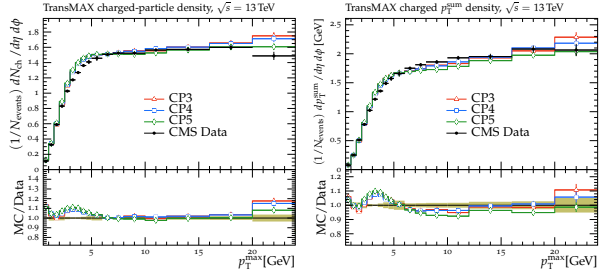
\includegraphics[width=0.8\textwidth]{{img/CPdistributions.png}}
	\caption{The evolution of the charged-particles density (left) and of the scalar-$p_T$ sum density of charged particles (right) as a function of the energy scale for the scattering (leading object $p_T$), the two distribution increase quite rapidly in the first bins than they saturate ($\approx 6-7\ \mathrm{GeV}$) the scalar-$p_T$ sum density increase a little bit more, for $p_T>$ but very slowly. The black dots are the experimental point and are compared to prediction with CMS \textsc{pythia} tunes: CP3, CP4 and CP5; they are described with more details in the next chapter. Figure from \cite{CPtunes}.}
	\label{fig:CPtransmax_evolution_with_energy}
\end{figure}

Now we want to look for the sensitivity of these observables to some \textsc{Pythia8} parameters. In figure \figRef{fig:CP5onlyPT0} is shown the effect of the MPI on booth the distributions shown before. The amount of the MPI is related to the value of $p_{T0}$: an high value of $p_{T0}$ is related to less MPI (blue line) and an higher value to a major contribution from the the MPI (red line).

\begin{figure}[!ht]
	\centering
	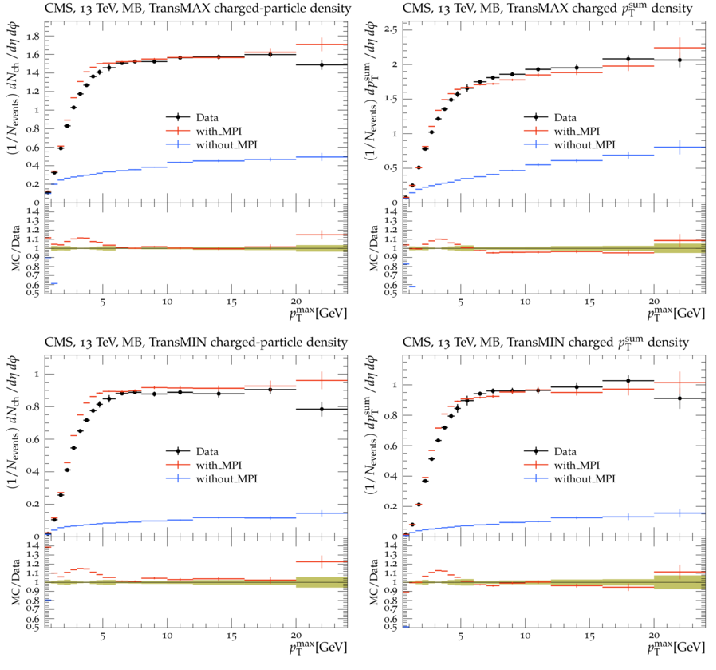
\includegraphics[width=0.8\textwidth]{{img/CP5_with_without_MPI.pdf}}
	\caption{This image shows the effect of the MPI in the transMAX and TransMin regions. The contribution of the parton shower alone can't explain the contributions of the underlying event in these two regions (blue line) the introduction of the contribution from the MPI is necessary (red line). The two simulations are compared to the data from \cite{CMS-PAS-FSQ-15-007}.}
	\label{fig:CP5onlyPT0}
\end{figure}

Another important observation that was also pointed out in the \chapRef{sec:BasicConcepts} is that the amount of activity in the two transverse regions is also dependent on the center-of-mass energy. This evolution is shown in \figRef{fig:CPECMdep} for two different energy. The amount of MPI increase with $\sqrt{s}$ that was expected from the evolution of the PDF with the energy of the collision: the hadrons become denser-packed when probed to higher energies.

\begin{figure}[!ht]
	\centering
	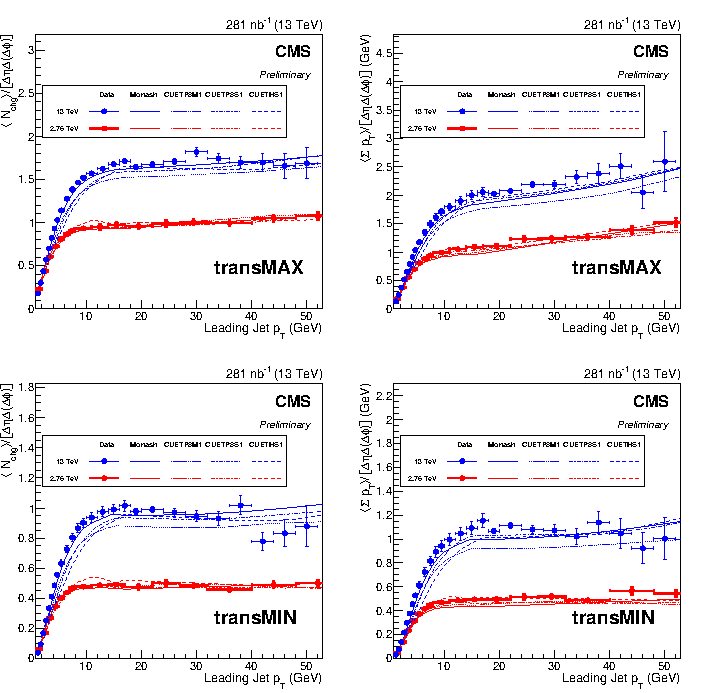
\includegraphics[width=0.85\textwidth]{{img/CPECMdep.pdf}}
	\caption{The charged particle density in the transMAX (upper left) and transMIN (lower left) regions and of the charged particle $p_T$-sum in the transMAX (upper right) and the transMIN (lower right) regions evolution as function of the center-of-mass energy is shown. The red ones are the data for $\sqrt{s}=2.76$ and the blue ones for $\sqrt{s}=13$ and these are compare to different CMS tunes. Figure from \cite{CMS-PAS-FSQ-15-007}}
	\label{fig:CPECMdep}
\end{figure}


